% --- FRAME 1: ICECUBE OVERVIEW ---
\begin{frame}{The IceCube Observatory and NGC 1068}
    \begin{columns}[T] % 'T' allinea il contenuto in alto
        
        % Prima colonna: IceCube
        \begin{column}{0.5\textwidth}
            \centering
            % keepaspectratio impedisce che l'immagine si deformi
            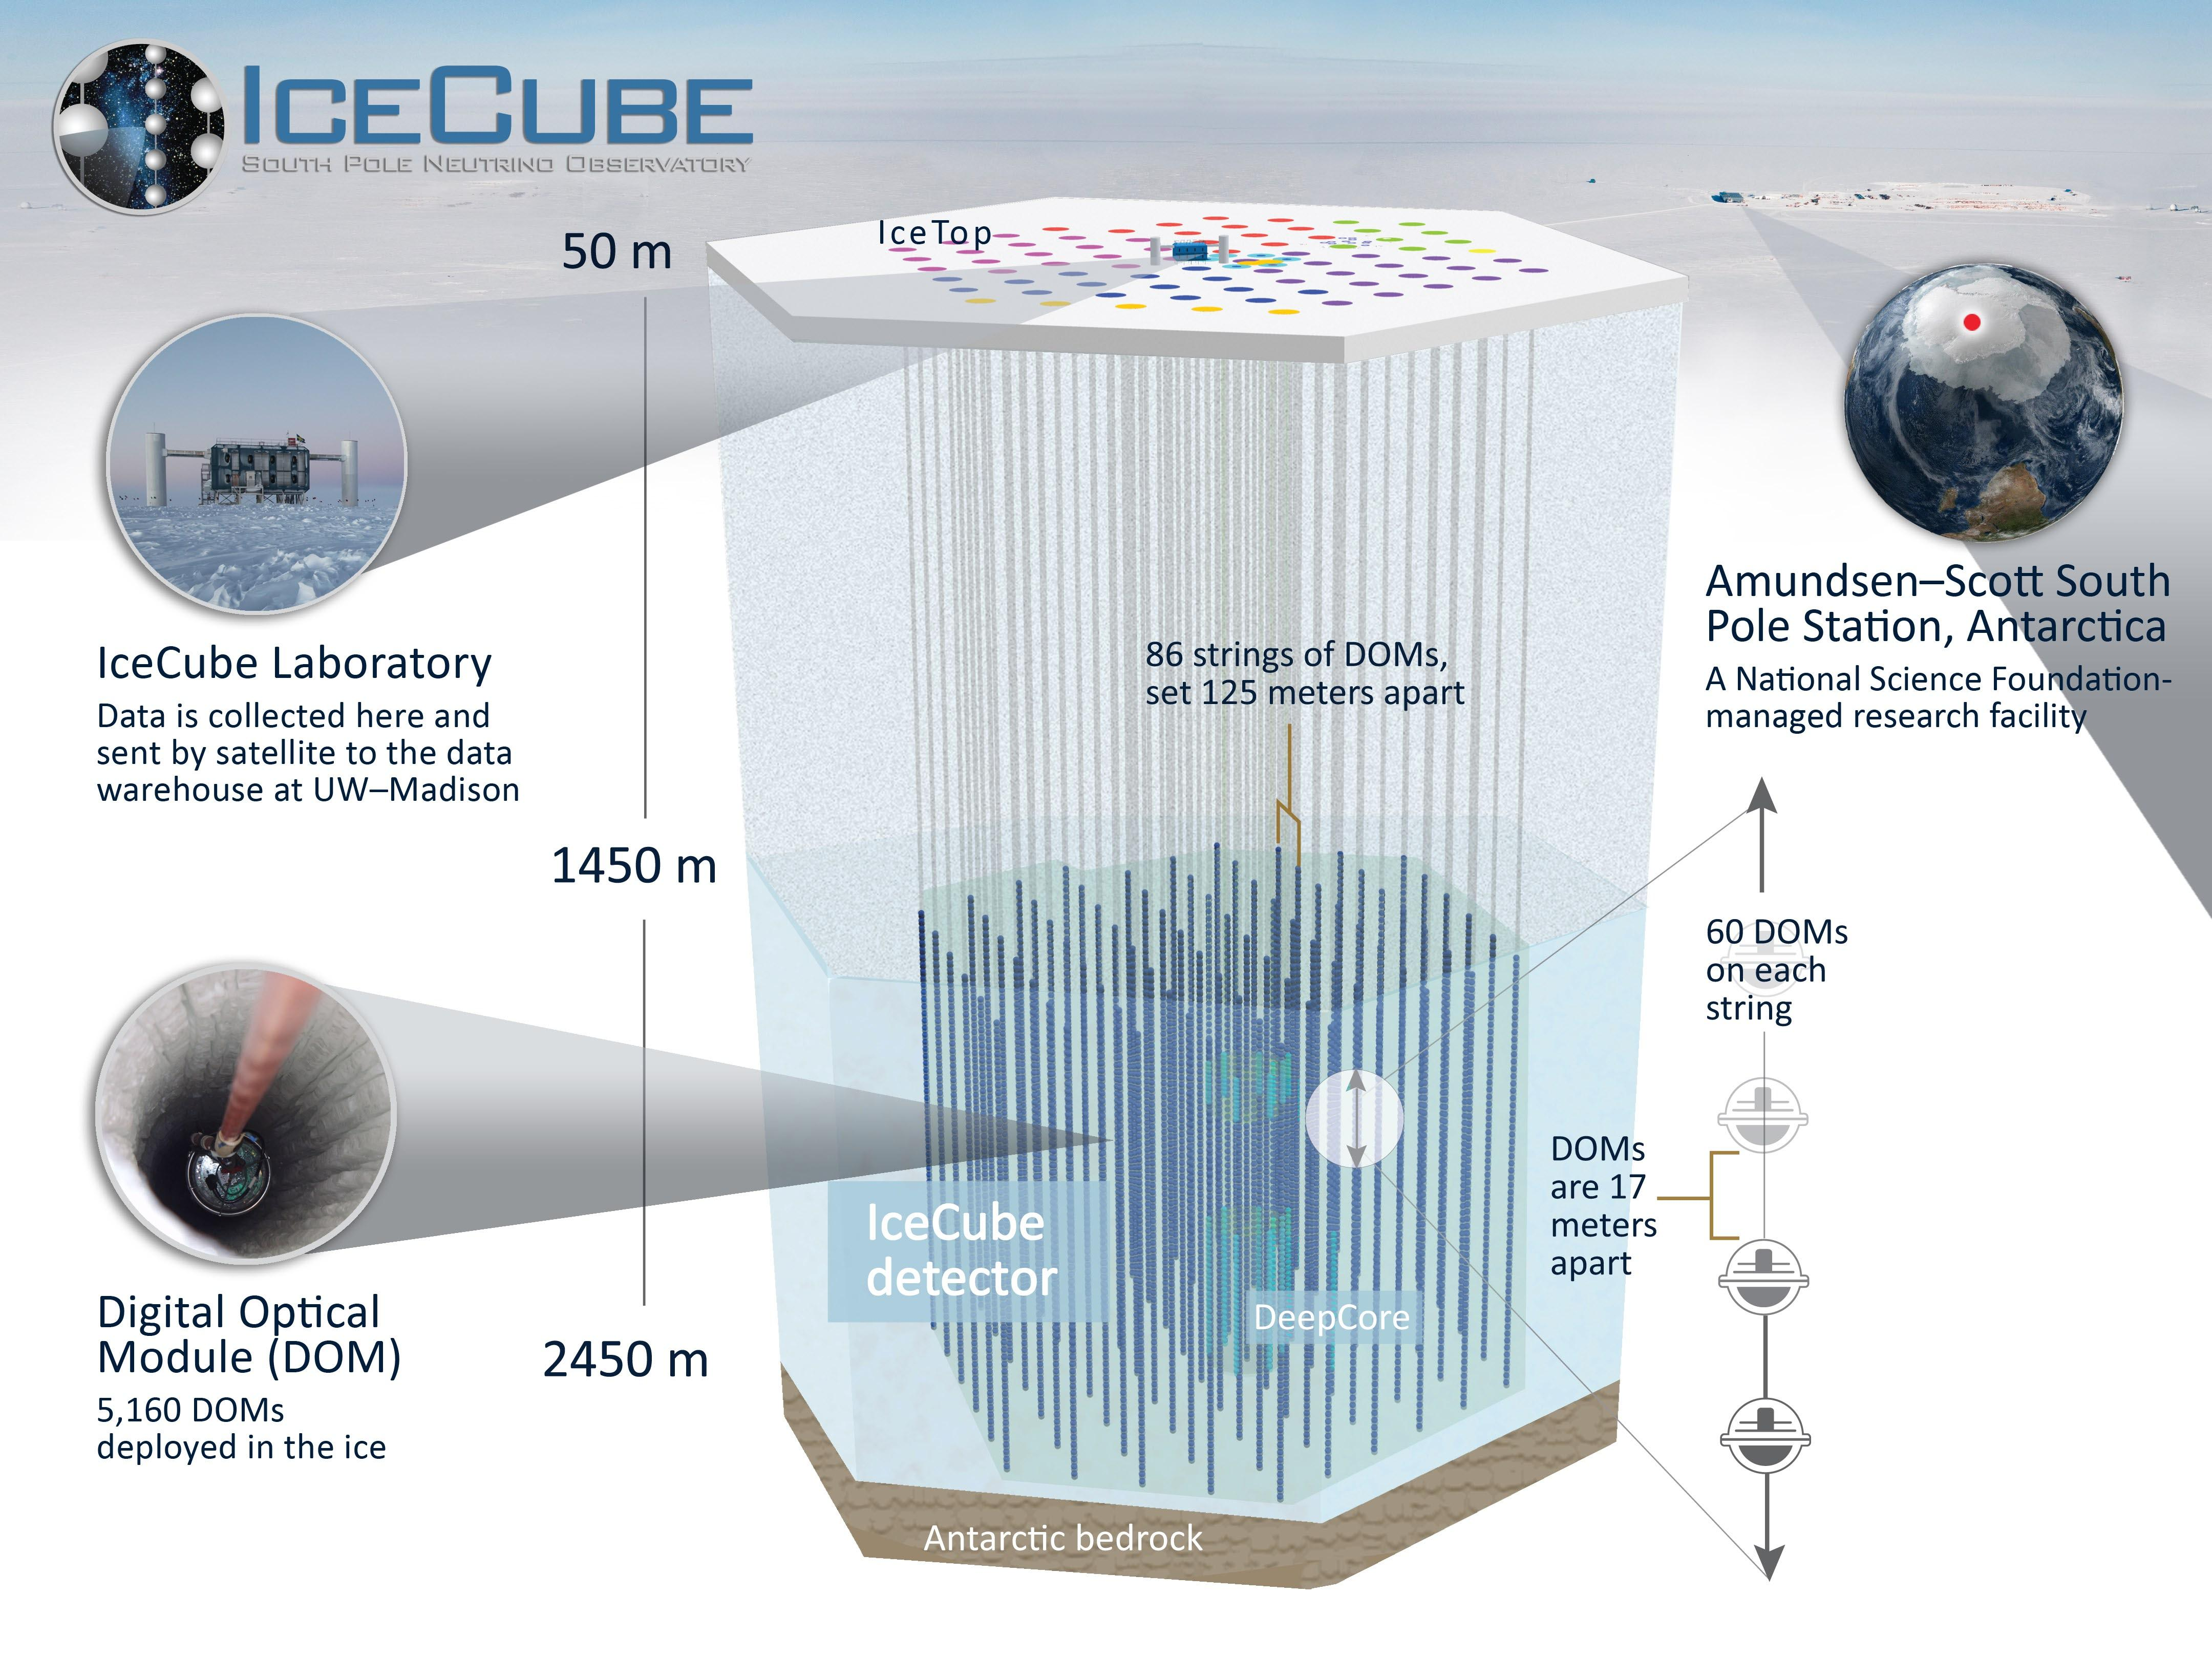
\includegraphics[width=\textwidth, keepaspectratio]{Immagini/icecube_detector.jpg}
            
            \vspace{0.47cm} % Aggiunge un po' di respiro tra immagine e link
            \tiny{\href{https://icecube.wisc.edu/science/icecube/}{Source: icecube.wisc.edu}}
        \end{column}
        
        % Seconda colonna: NGC 1068 (NASA)
        \begin{column}{0.5\textwidth}
            \centering
            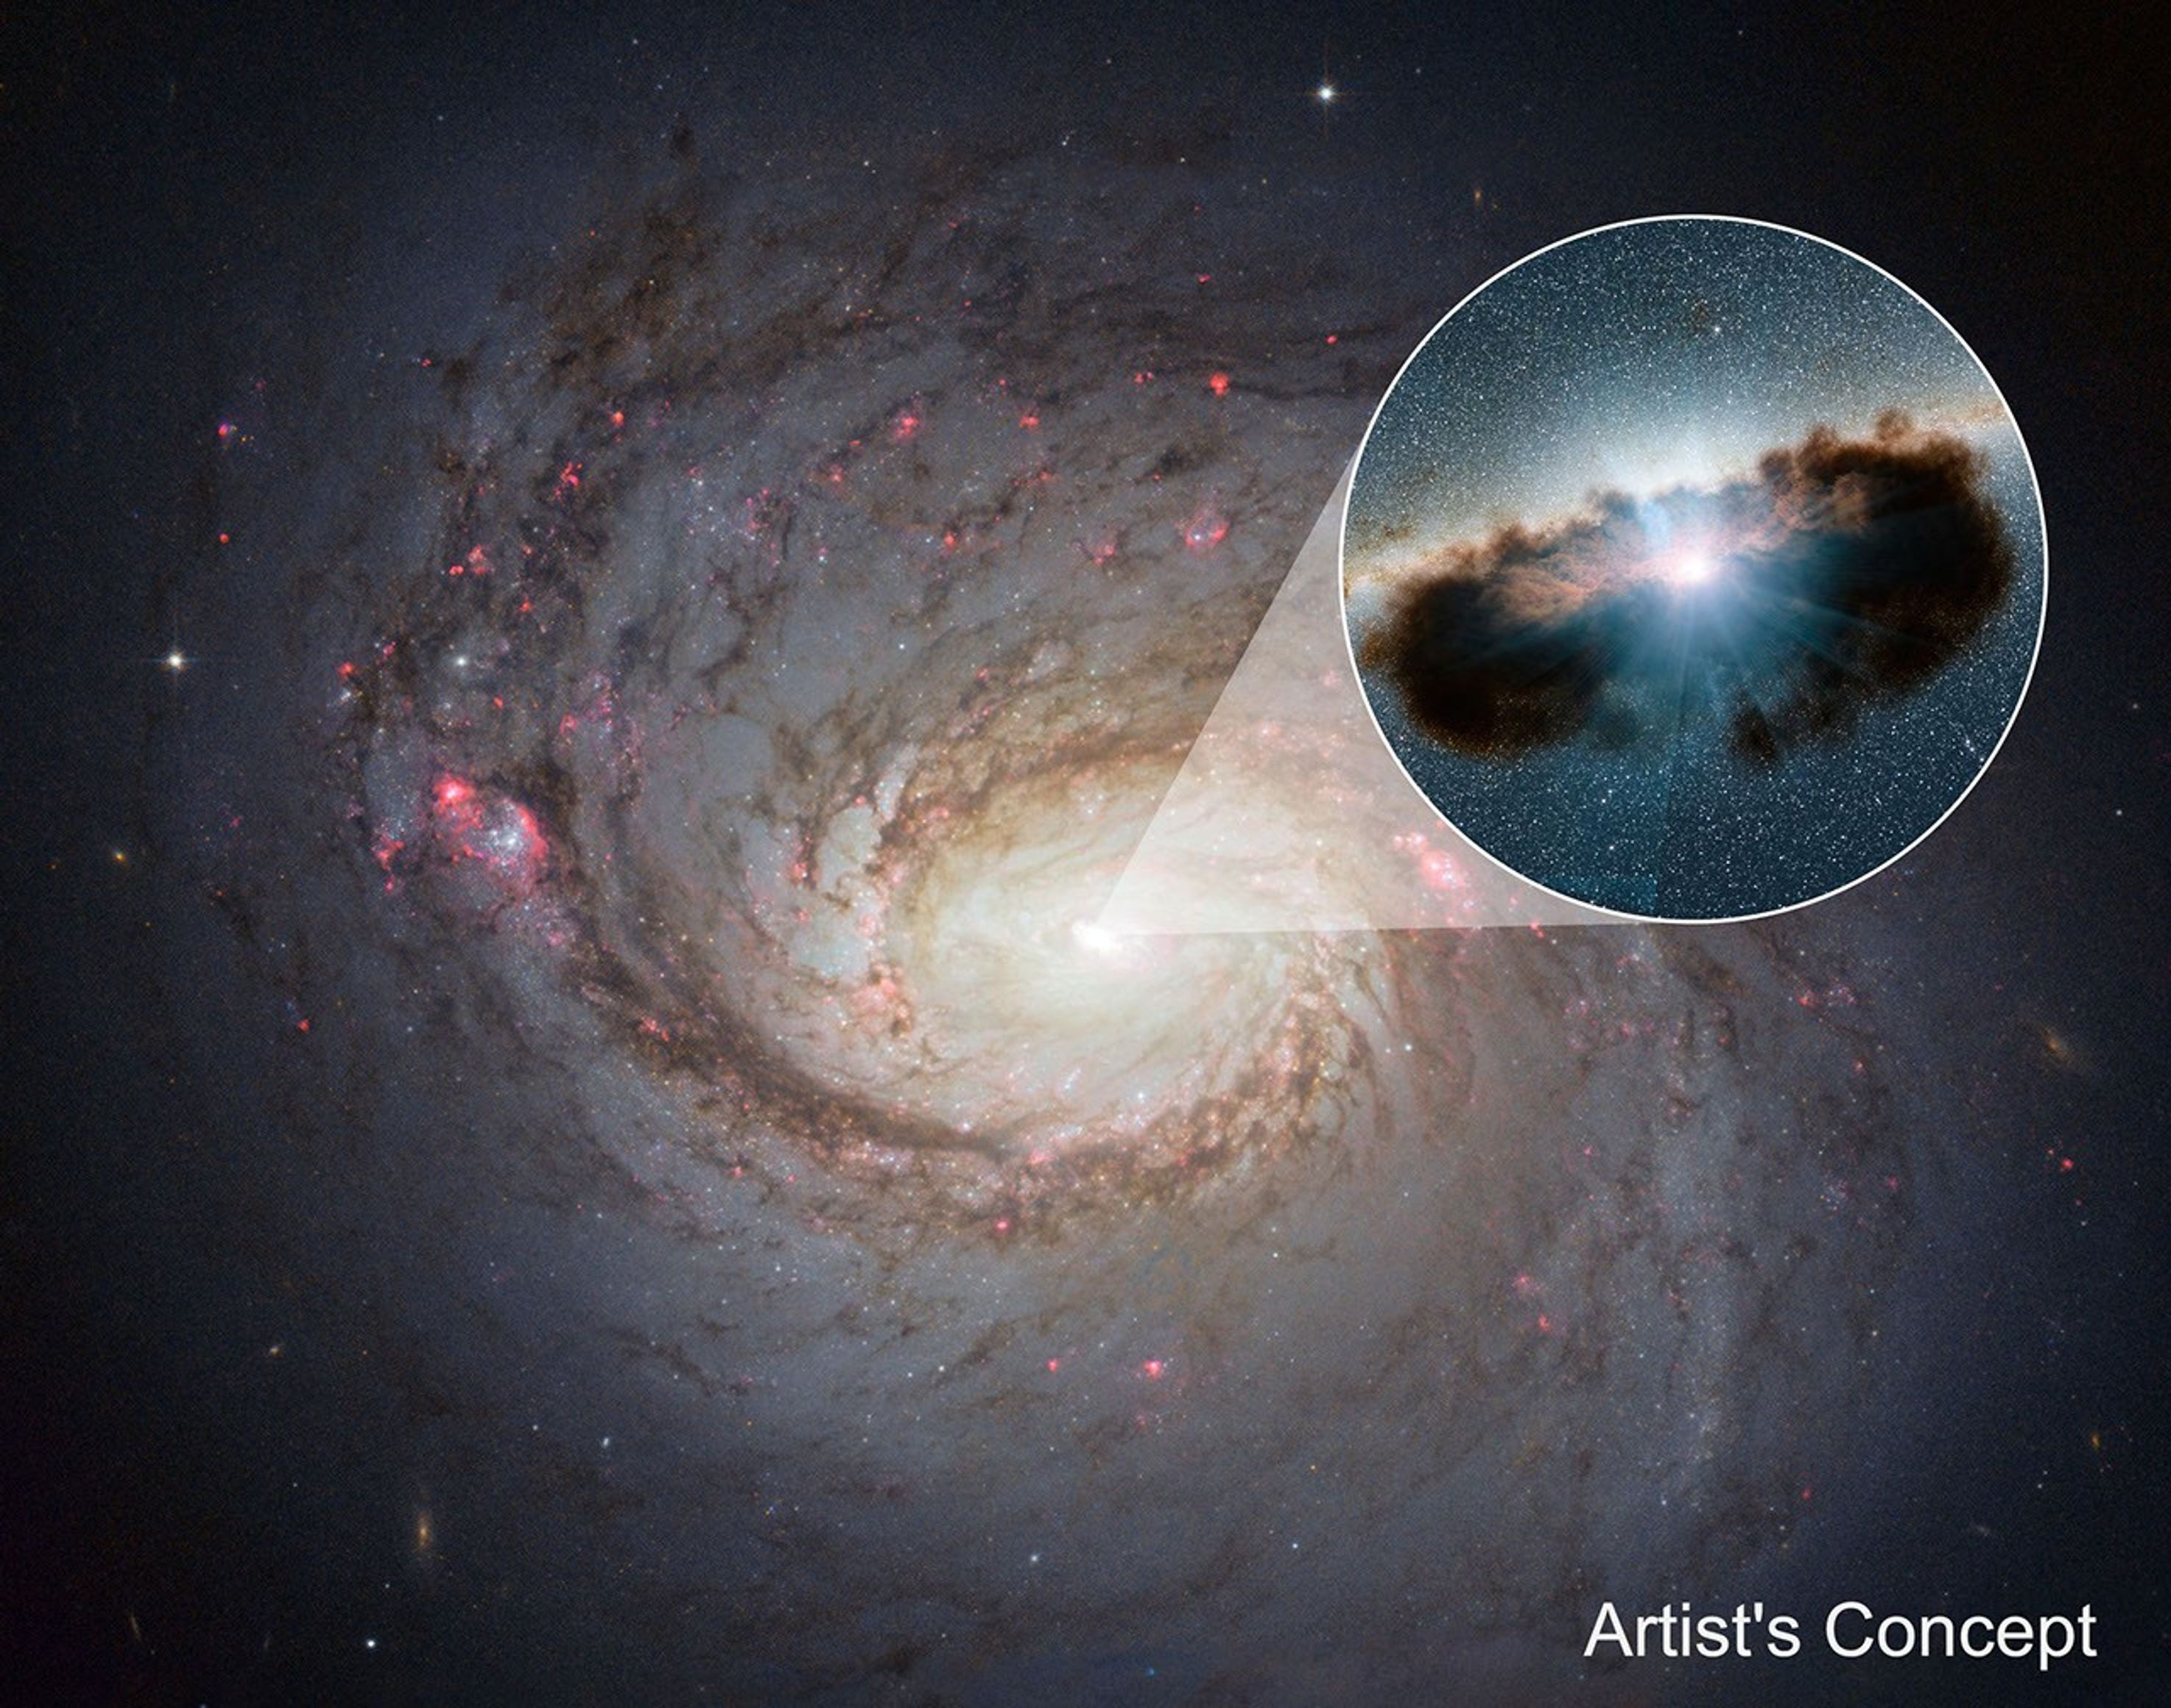
\includegraphics[width=\textwidth, keepaspectratio]{Immagini/nasa.jpg}
            
            \vspace{0.2cm}
            \tiny{\href{https://science.nasa.gov/photojournal/hidden-lair-at-the-heart-of-galaxy-ngc-1068/}{Source: science.nasa.gov}}
        \end{column}
        
    \end{columns}
\end{frame}

\begin{frame}{Dataset Selection \& Spatial Cuts}
    
    % Testo discorsivo conciso in alto
    The \textbf{Tracks dataset} provides the excellent angular resolution ($\lesssim 1^\circ$) required for point-source astronomy. 
    
    The analysis is strictly confined to a narrow \textbf{declination band} ($\delta \in [-3^\circ, +5^\circ]$).
    
    % Immagine in grande in basso
    \begin{figure}
        \centering
        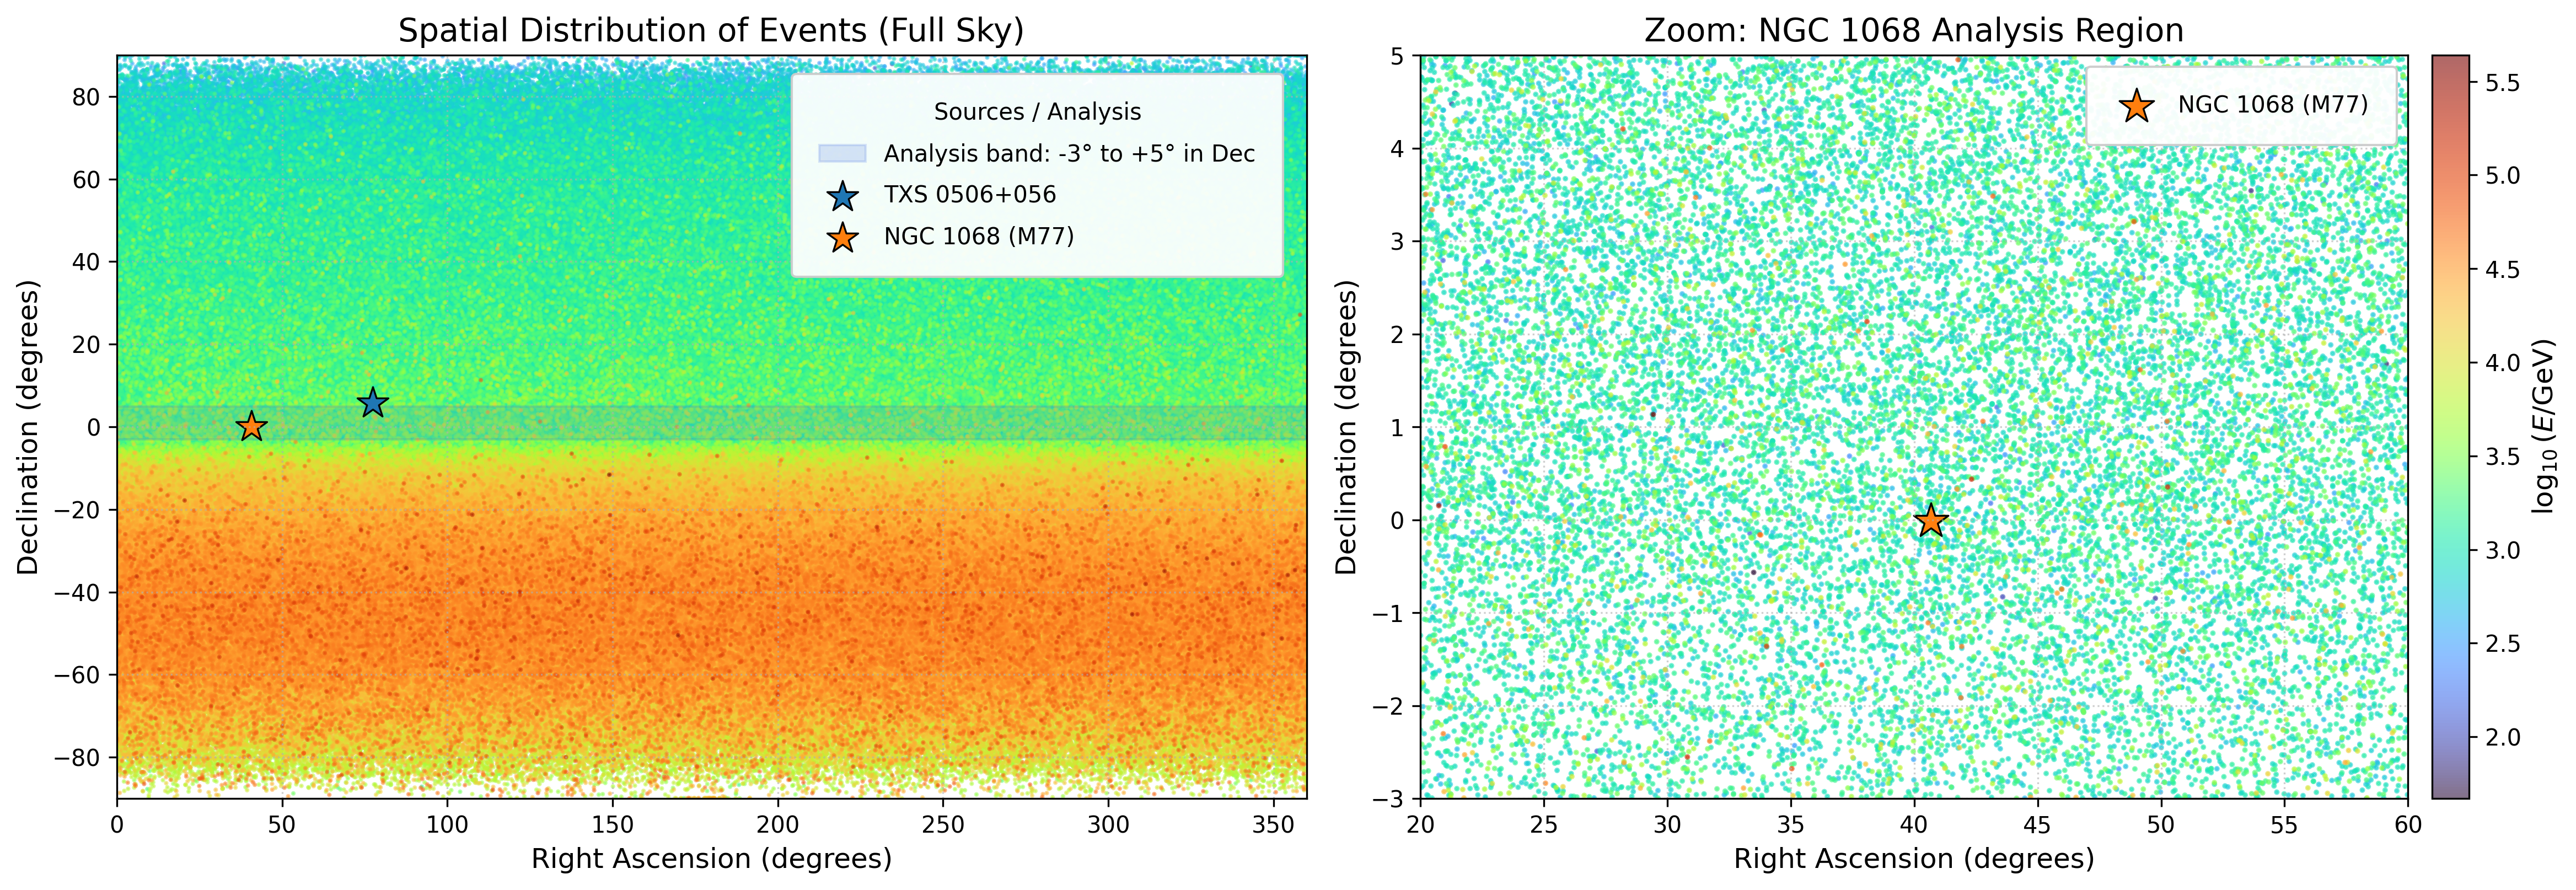
\includegraphics[width=0.99\textwidth, keepaspectratio]{Immagini/02_skymap_events_With_Two_sources.png}
    \end{figure}
    
    
\end{frame}

\begin{frame}{Physical Motivation: The Declination Band}
    \begin{columns}[c]
        
        % Colonna Immagine
        \begin{column}{0.5\textwidth}
            \centering
            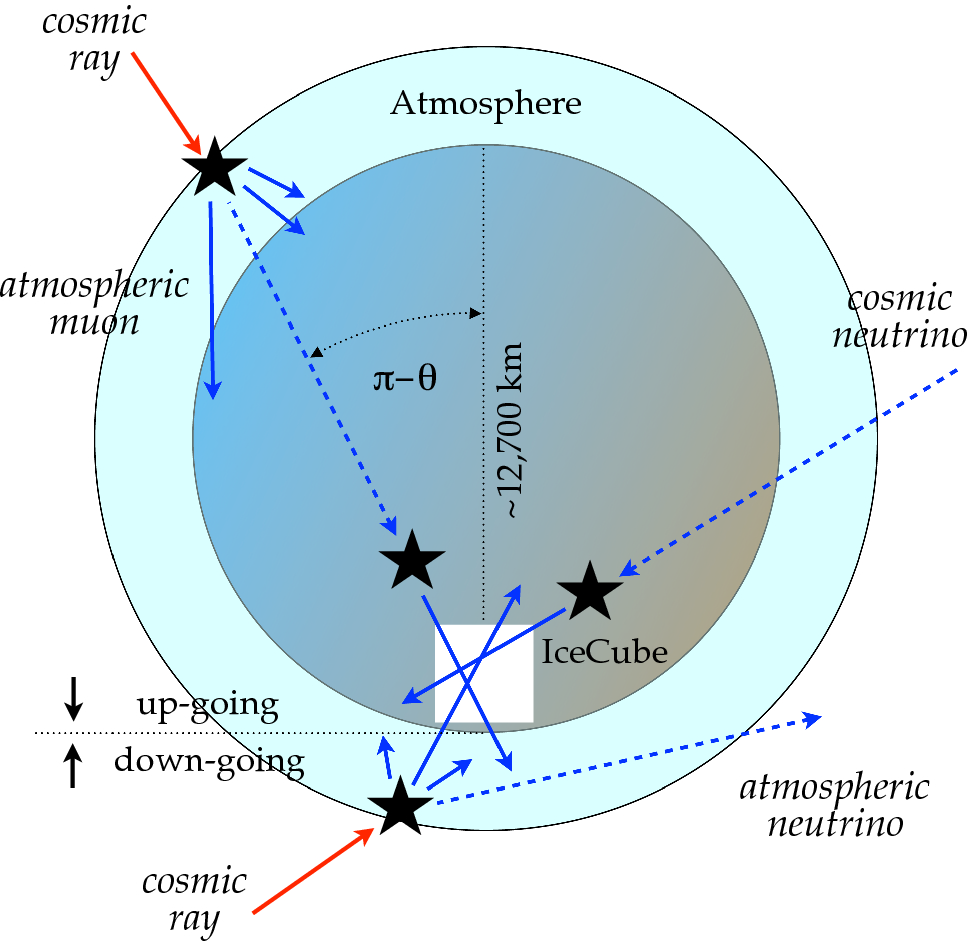
\includegraphics[width=0.85\textwidth, keepaspectratio]{Immagini/scheme.png}\\
            \vspace{0.1cm}
            \tiny{\href{https://link.springer.com/article/10.1140/epjc/s10052-018-6369-9/figures/3}{Source: link.springer.com}}
        \end{column}
        
        % Colonna Testo
        \begin{column}{0.48\textwidth}
            \textbf{1. Declination Band}
            \begin{itemize}
                \item \textbf{Target:} NGC 1068 ($\delta \approx -0.06^\circ$)
                \item \textbf{Window:} $\delta \in [-3^\circ, +5^\circ]$
                \item[$\rightarrow$] Uniform detector acceptance
            \end{itemize}
            
            \vspace{0.5cm}
            
            \textbf{2. Background Estimation}
            \begin{itemize}
                \item \textbf{Method:} RA Scrambling
                \item \textbf{Action:} Fix $\delta$, randomize RA
                \item[$\rightarrow$] Data-driven background (incorporates exposure)
            \end{itemize}
        \end{column}
        
    \end{columns}
\end{frame}

\begin{frame}{First naive signal search for NGC 1068}
    \begin{columns}[c] % Allineamento verticale al centro
        
        % Colonna di sinistra: Immagine
        \begin{column}{0.58\textwidth}
            \centering
            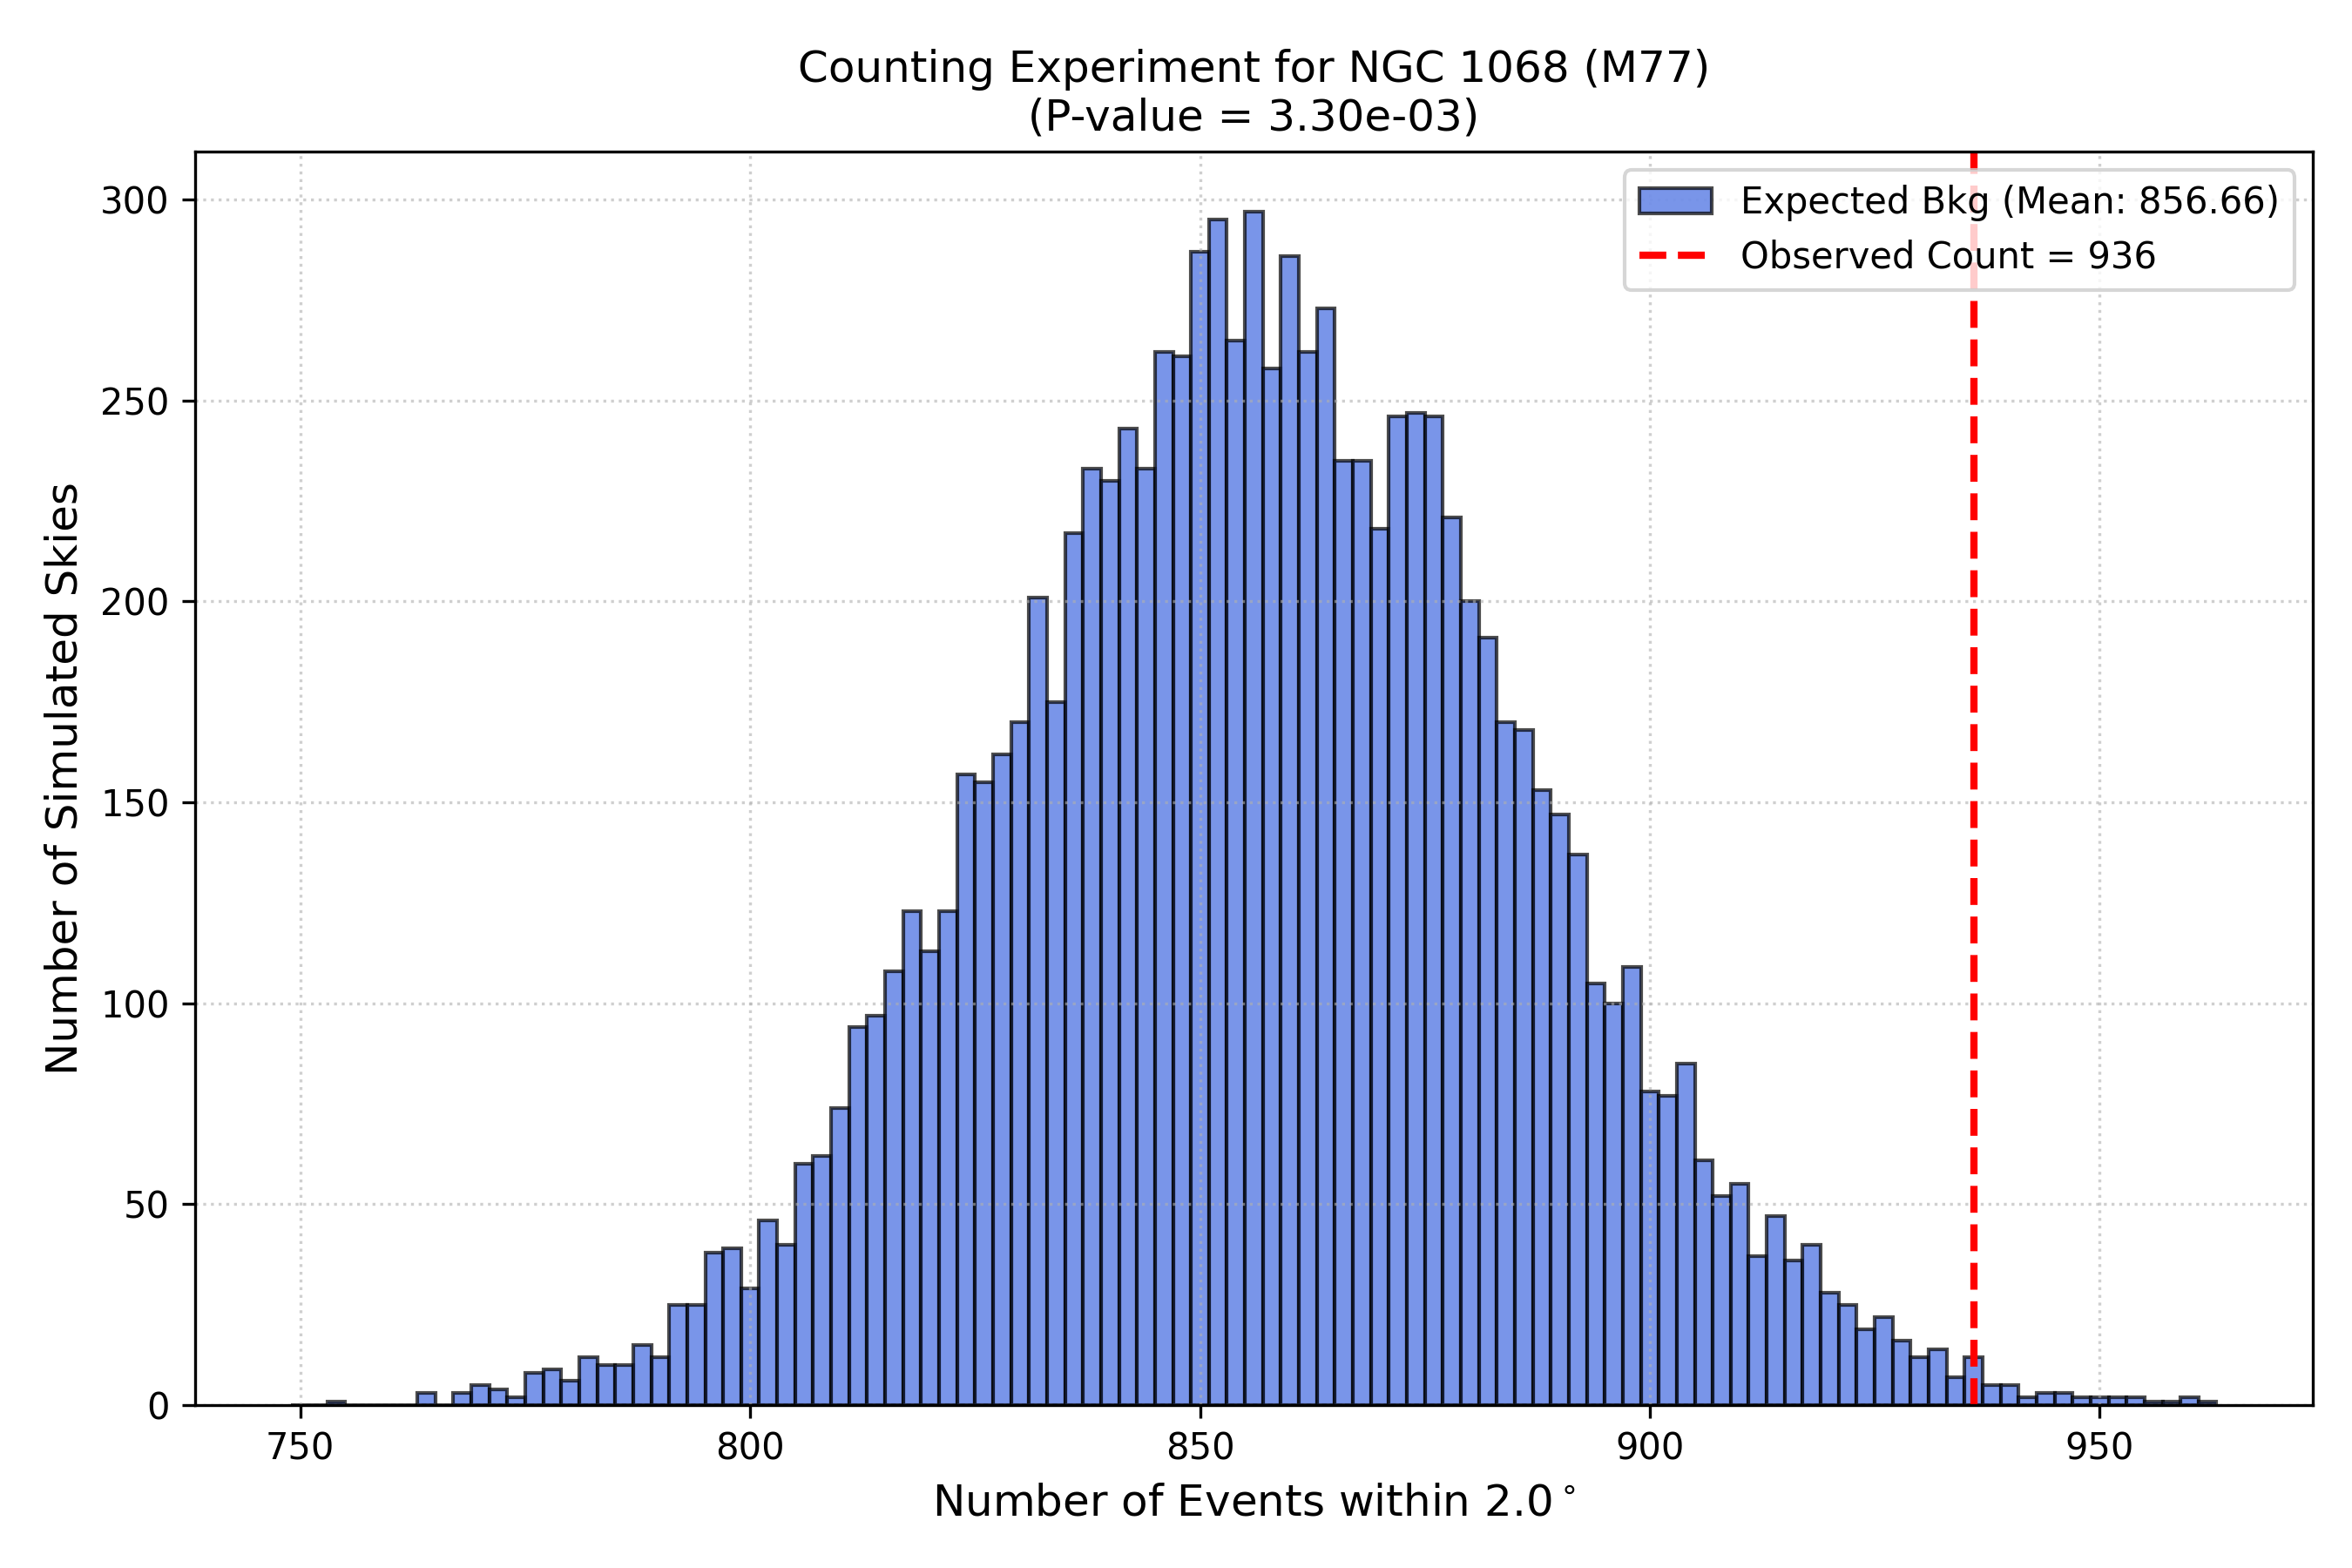
\includegraphics[width=\textwidth]{Immagini/02b_binned_scrambling_counting.png}
        \end{column}
        
        % Colonna di destra: Box dei risultati
        \begin{column}{0.42\textwidth}
            
            % Puoi usare "alertblock" al posto di "block" se vuoi farlo risaltare di più
            \begin{block}{Counting Analysis Results}
                \small % Rimpicciolisce leggermente il testo per non farlo sbordare
                \begin{itemize}
                    \setlength{\itemsep}{0.3em} % Dà un po' di respiro tra le righe
                    \item \textbf{Simulated Skies:} $10^4$
                    \item \textbf{Observed Events:} $936$
                    \item \textbf{Expected Bkg:} $856.7 \pm 29.1$
                    \item \textbf{Excess Events:} $79.3$
                    \item \textbf{p-value:} $3.3 \times 10^{-3}$
                    \item \textbf{Significance:} $2.72\sigma$
                \end{itemize}
            \end{block}
            
        \end{column}
        
    \end{columns}
\end{frame}

\begin{frame}{Unbinned Spatial Likelihood}

    % Formula Generale
    \textbf{Mathematical Framework}
    \begin{equation*}
        \mathcal{L}(n_s) = \prod_{i=1}^{N} \left[ \frac{n_s}{N} \mathcal{S}_i + \left(1 - \frac{n_s}{N}\right) \mathcal{B}_i \right]
    \end{equation*}
    \vspace{-0.3cm}
    \begin{itemize}
        \item $N$: Total events in the declination band.
        \item $n_s$: Number of signal events (\textit{free parameter} to be maximized).
    \end{itemize}

    \vspace{0.3cm}

    % Colonne per le PDF
    \textbf{Probability Density Functions (PDFs)}
    \vspace{0.2cm}
    \begin{columns}[t]
        
        % Colonna Segnale
        \begin{column}{0.48\textwidth}
            \centering{\textbf{Signal PDF ($\mathcal{S}_i$)}}
            \begin{equation*}
                \mathcal{S}_i = \frac{1}{2\pi\sigma_i^2} \exp\left(-\frac{\psi_i^2}{2\sigma_i^2}\right)
            \end{equation*}
        \end{column}
        
        % Colonna Fondo
        \begin{column}{0.48\textwidth}
            \centering{\textbf{Background PDF ($\mathcal{B}_i$)}}
            \begin{equation*}
                \mathcal{B}_i(\delta_i) = \frac{1}{\Delta \Omega_{\text{band}}} = \frac{1}{2\pi (\sin \delta_{\text{max}} - \sin \delta_{\text{min}})}
            \end{equation*}
        \end{column}
        
    \end{columns}
\end{frame}

\begin{frame}{Results: Unbinned Spatial Likelihood Scan}
    \begin{columns}[c]
        
        % Colonna Sinistra: Il Grafico
        \begin{column}{0.55\textwidth}
            \vspace{-0.5cm}
            \begin{figure}
                \centering
                % Inserisci qui l'immagine del tuo likelihood scan
                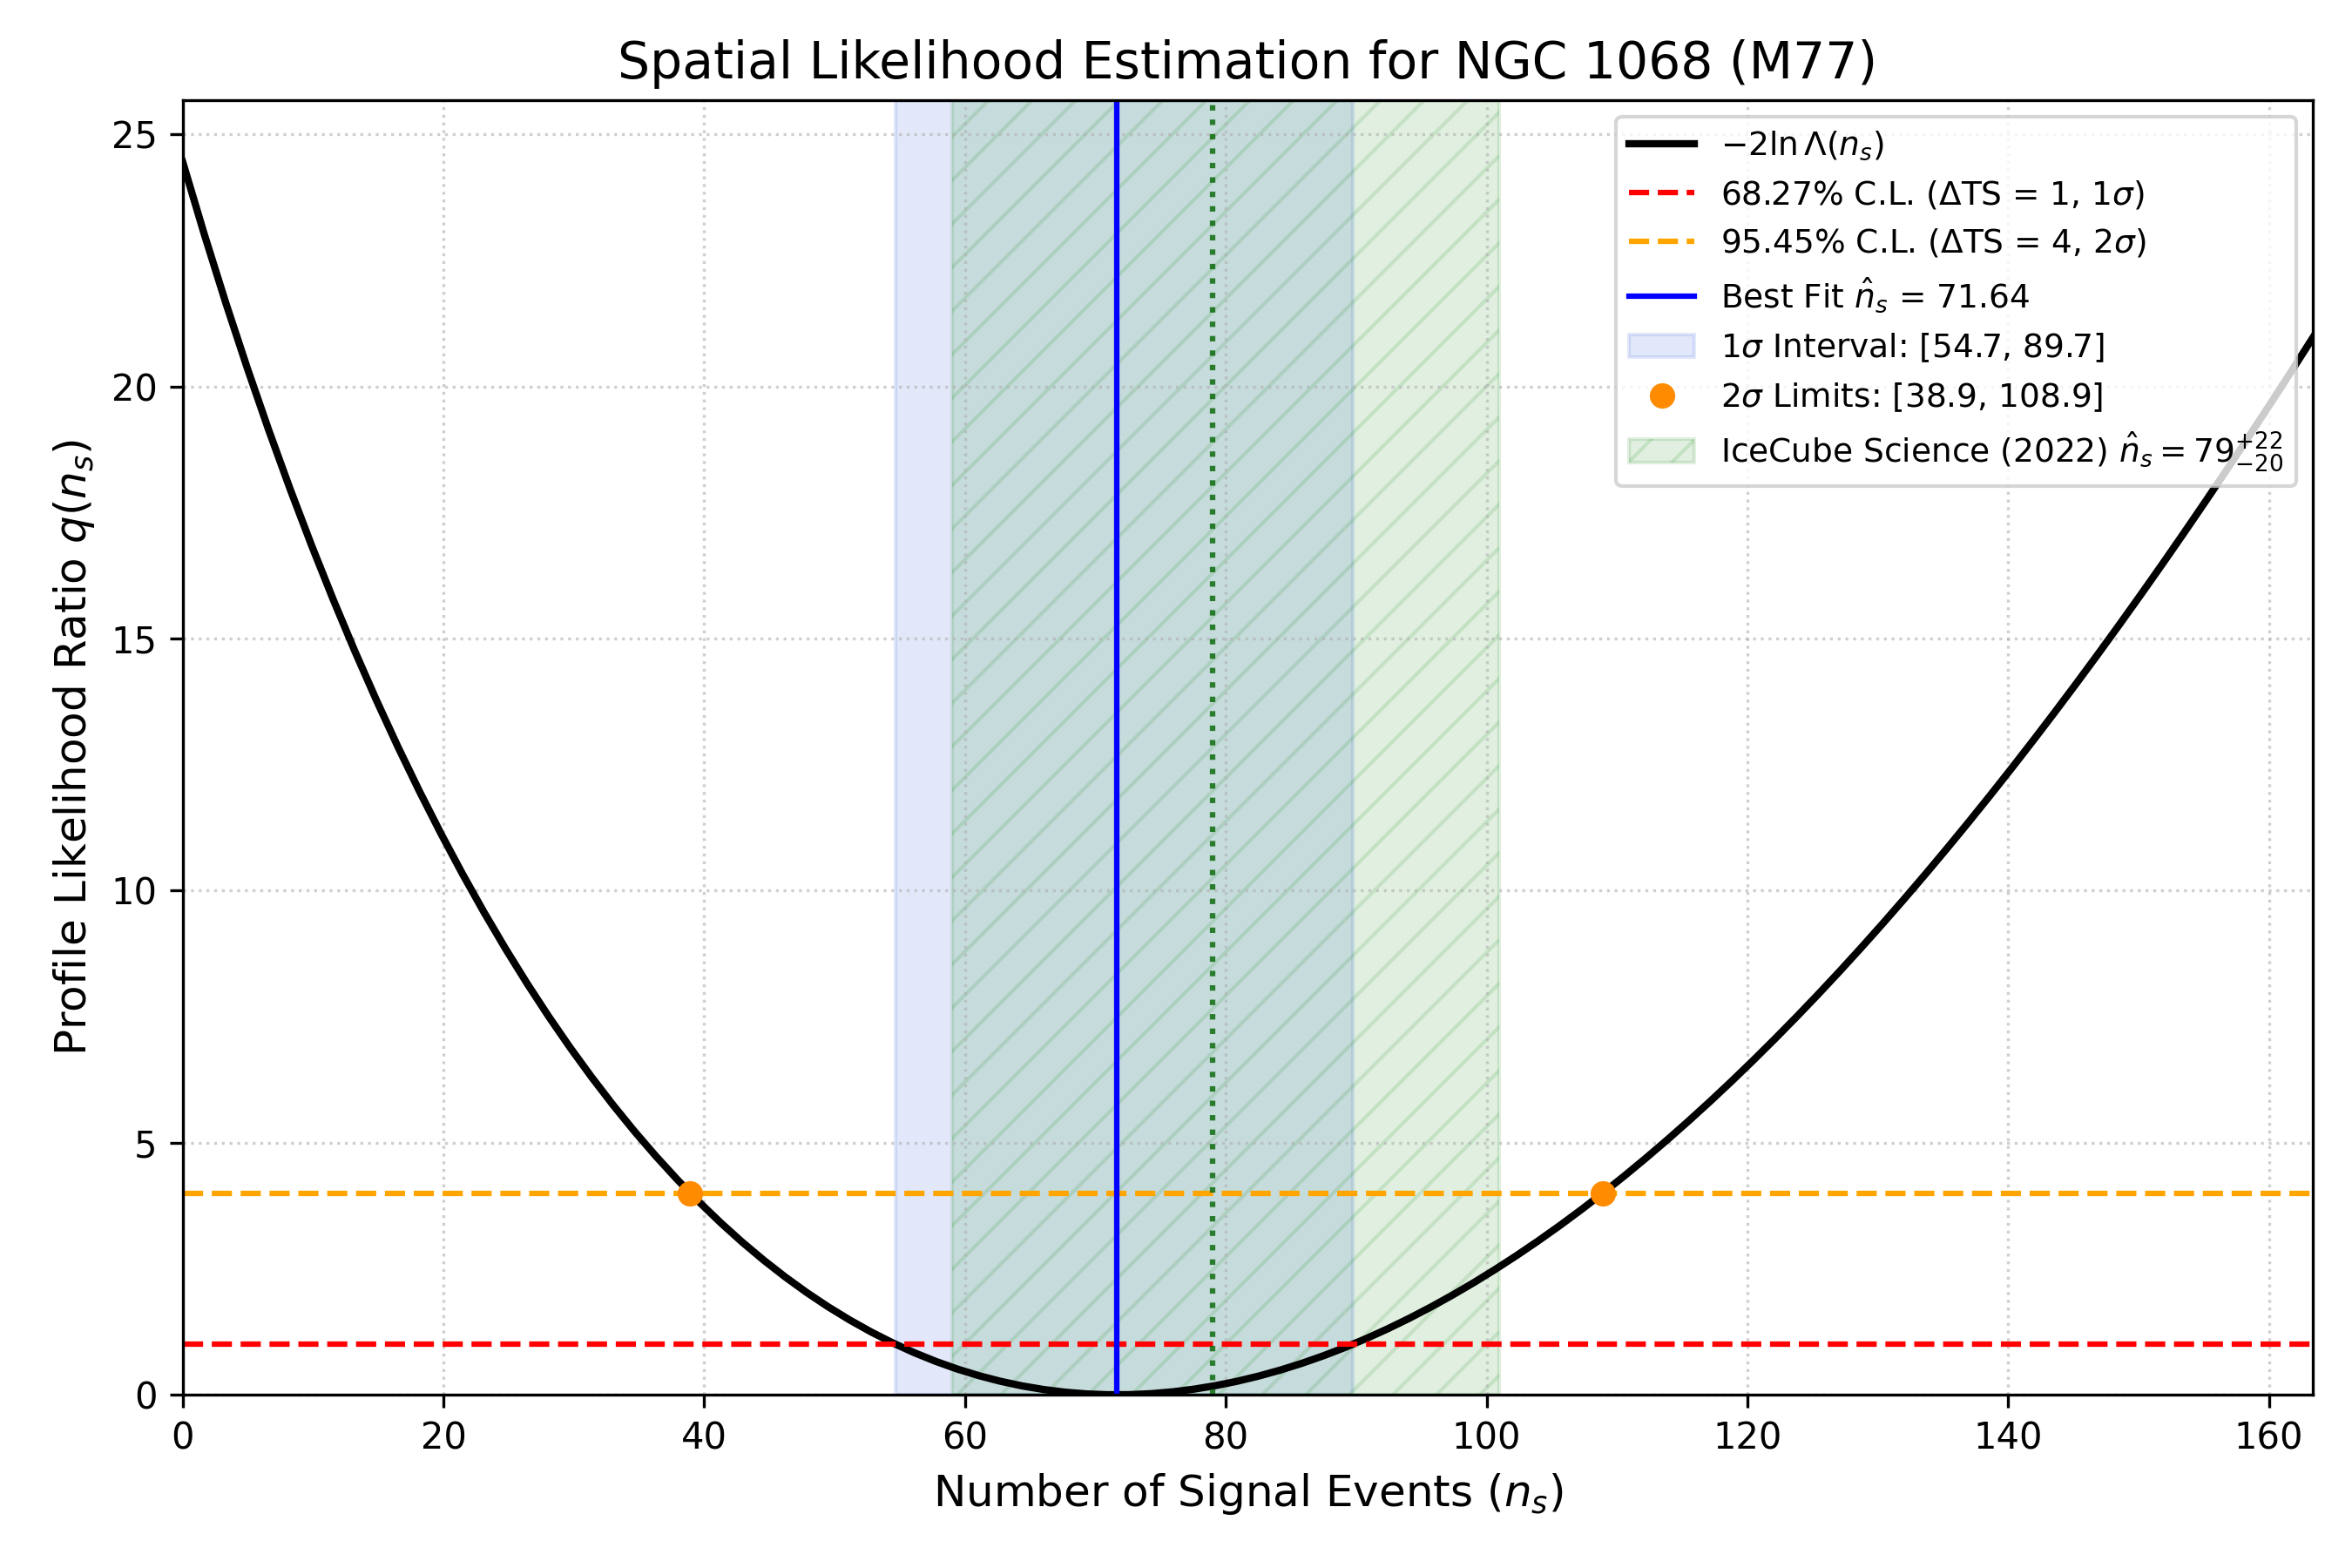
\includegraphics[width=\textwidth]{Immagini/03_likelihood_scan.png}
            \end{figure}
        \end{column}
        
        % Colonna Destra: I Dati Scientifici
        \begin{column}{0.48\textwidth}
            
            \begin{block}{Best-Fit Signal}
                \begin{itemize}
                    \item $\hat{n}_s = 71.64_{-16.94}^{+18.08}$ \hfill ($1\sigma$ C.L.)
                    \item $2\sigma$ interval: $[38.94, 108.91]$
                \end{itemize}
            \end{block}
            
            \begin{block}{Statistical Significance}
                \begin{itemize}
                    \item $TS_{\text{obs}} = 24.46$
                    \item Local p-value $< 2.0 \times 10^{-4}$ \\
                    \small{(0 background fluctuations in 5000 trials)}
                    \item Significance: $\ge 3.54\sigma$
                \end{itemize}
            \end{block}
            
        \end{column}
        
    \end{columns}
\end{frame}


\begin{frame}{Future Directions}
    \textbf{Enhancing the Likelihood Model:}
    \begin{itemize}
        \item \textbf{Energy Integration:} Add energy-dependent PDFs (e.g., injecting an $E^{-3.2}$ source spectrum) to boost signal-background discrimination.
        \item \textbf{Source Morphology:} Test extended spatial models instead of a strict point-source approximation.
    \end{itemize}
    
    \vspace{0.5cm}
    
    \textbf{Astrophysical Context:}
    \begin{itemize}
        \item \textbf{Time-Dependent Search:} Investigate temporal correlations with known AGN flaring activities.
        \item \textbf{Multi-Messenger Approach:} Cross-correlate neutrino arrivals with X-ray and $\gamma$-ray astronomical catalogs.
    \end{itemize}
\end{frame}


\begin{frame}{Conclusions}
    \begin{itemize}
        \item[\checkmark] \textbf{Methodology:} Successfully implemented a complete, unbinned spatial likelihood pipeline using a data-driven background (RA scrambling).
        
        \vspace{0.3cm}
        
        \item[\checkmark] \textbf{Detection:} Found a statistically significant neutrino excess ($\ge 3.54\sigma$) originating from the NGC 1068 coordinates.
        
        \vspace{0.3cm}
        
        \item[\checkmark] \textbf{Consistency:} Despite the "spatial-only" simplification, the estimated signal ($\hat{n}_s \approx 72$) is remarkably consistent with the complex official IceCube findings.
    \end{itemize}
\end{frame}